\documentclass{article}
\usepackage[a4paper, total={7in, 9.5in}]{geometry}
\usepackage{amsmath,amsfonts,amsthm,amssymb,graphicx,float, setspace, bm}
\usepackage[utf8]{inputenc}
\usepackage{float}
\usepackage{titlesec}
\usepackage{setspace}
\usepackage{geometry}
\usepackage[style=numeric]{biblatex}
\usepackage[autostyle=true]{csquotes}
\usepackage{breqn}
\usepackage{subfig}
\usepackage[bottom]{footmisc}
\usepackage{adjustbox}
\usepackage{lipsum}
\usepackage{hyperref}
\usepackage[ruled,vlined]{algorithm2e}
\hypersetup{
    colorlinks=true,
    urlcolor=magenta
}
\usepackage[table,x11names]{xcolor}

\usepackage{xltabular}
\usepackage{multirow}
\usepackage{booktabs}


\renewcommand{\baselinestretch}{1.5} 
\setlength\parindent{0pt}
%----------------------------------------------------------------------------------------
%	START
%----------------------------------------------------------------------------------------

\newcommand{\horrule}[1]{\rule{\linewidth}{#1}}

\title{ \normalfont \normalsize 
\huge CPSC 532 - Homework 3}
\date{}
\author{Xiaoxuan Liang - 48131163}
\def\cond{\; | \;}

\begin{document}

\maketitle

Public GitHub repo: https://github.com/Xiaoxuan1121/CPSC532W/tree/main/a2
\begin{enumerate}
\item Program 1: the program has been run for 50000 times,  and the results are:
\begin{enumerate}
\item Importance Sampling:

\begin{figure}[!ht]
	\centering
	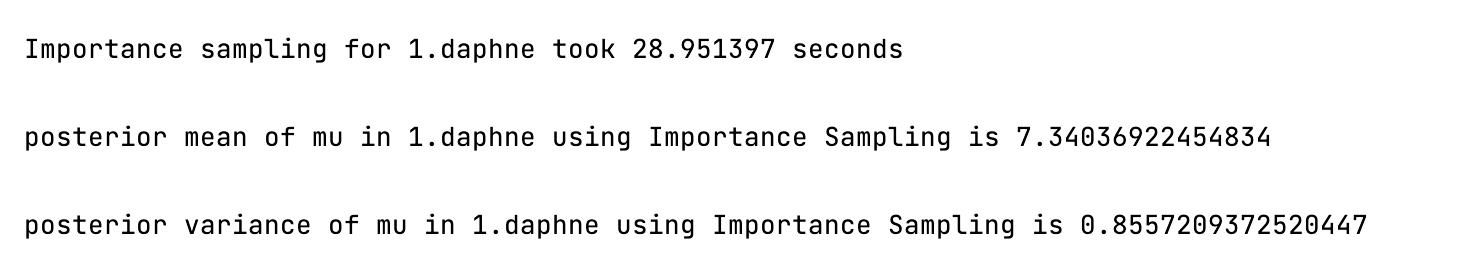
\includegraphics[scale=0.6]{../figs/IS/1_program_results}
\end{figure}

\begin{figure}[!ht]
	\centering
	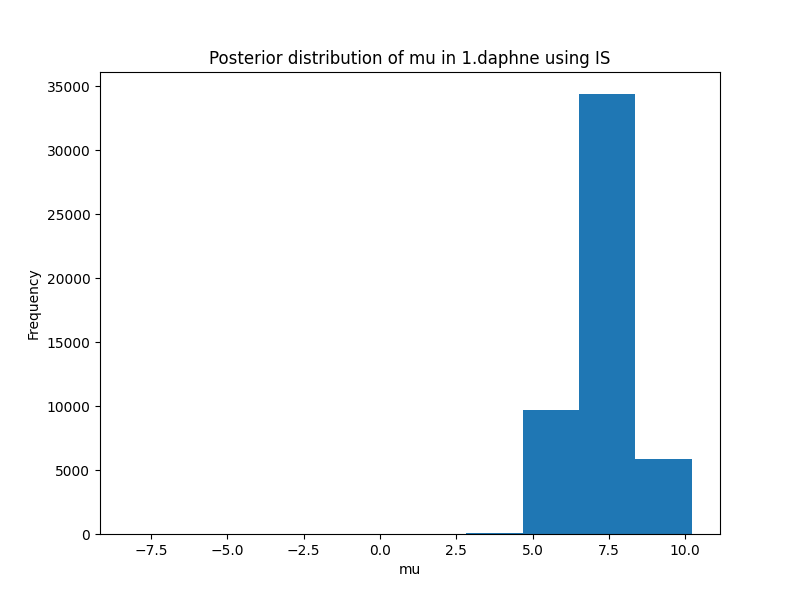
\includegraphics[scale=0.6]{../figs/IS/posterior_histogram_1_daphne}
\end{figure}

\newpage
\item MH Gibbs:

\begin{figure}[!ht]
	\centering
	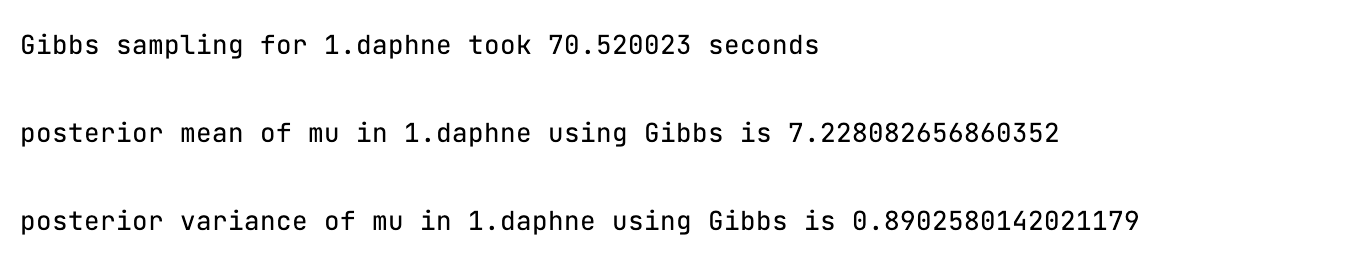
\includegraphics[scale=0.6]{../figs/Gibbs/1_program_results}
\end{figure}

\begin{figure}[!ht]
	\centering
	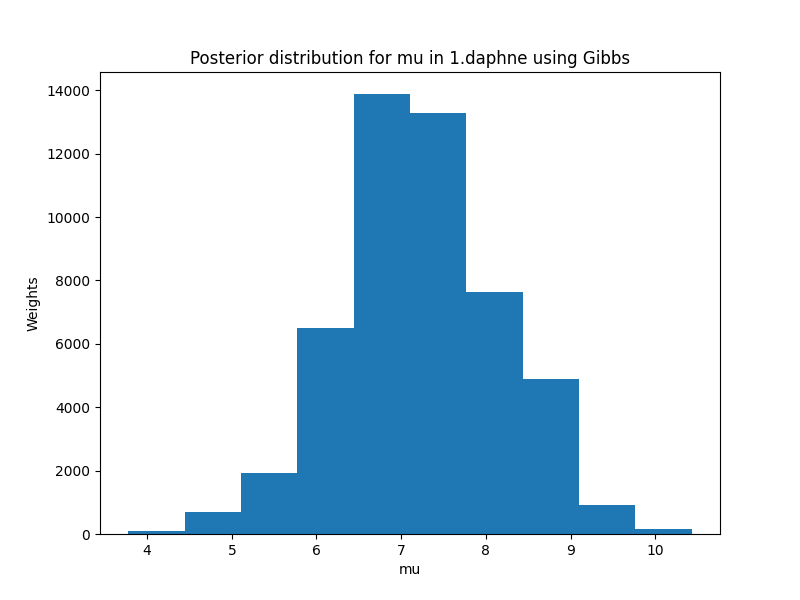
\includegraphics[scale=0.6]{../figs/Gibbs/posterior_histogram_1_daphne}
\end{figure}

\begin{figure}[!ht]
	\centering
	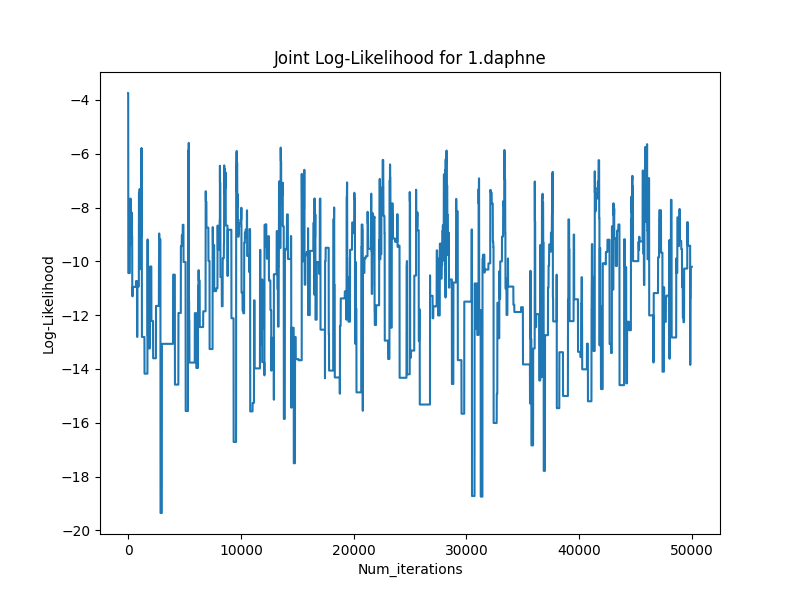
\includegraphics[scale=0.6]{../figs/Gibbs/joint_log_likelihood_1_daphne}
\end{figure}

\begin{figure}[!ht]
	\centering
	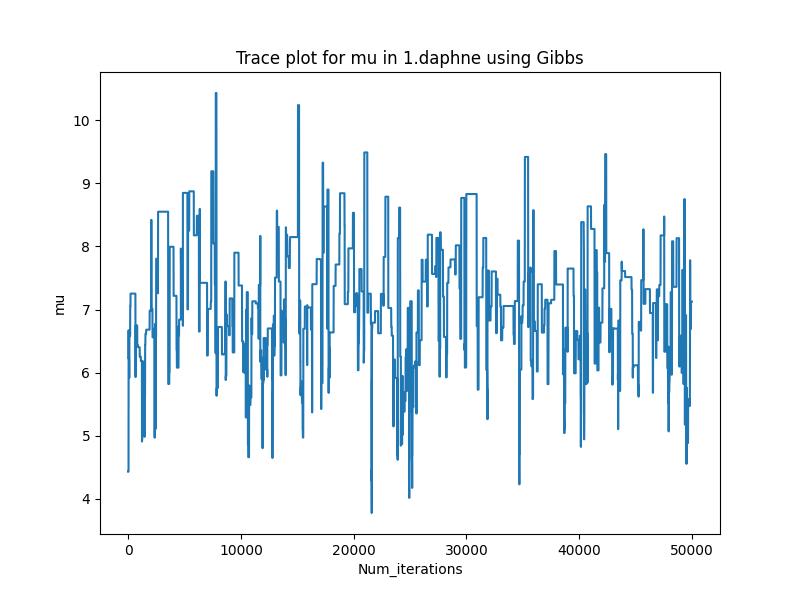
\includegraphics[scale=0.6]{../figs/Gibbs/trace_plot_1_daphne}
\end{figure}


\item HMC:

\begin{figure}[!ht]
	\centering
	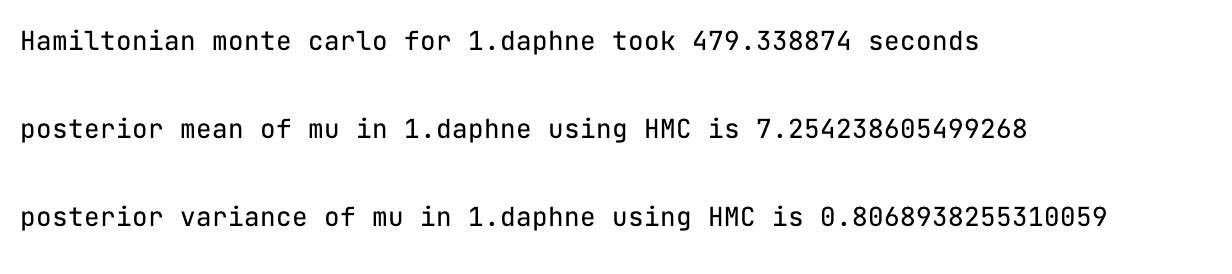
\includegraphics[scale=0.6]{../figs/HMC/1_program_results}
\end{figure}

\end{enumerate}
\end{enumerate}
\end{document}